\section{Initial concept and definitions}\label{sec:background}

%%I detta avsnitt redogör du för sådan kunskap som läsaren behöver för att förstå ditt arbete och ditt bidrag. Presentera fundamental kunskap som behövs för att förstå området och uppgiften. Till exempel kan du här redogöra för relevanta teorier och förklara begrepp du använder eller introducera matematisk notation. Skriv bakgrunden så att den som är väl insatt i området kan hoppa över den.

%\section{Background and related works}%
%\label{sec:bg}
In this section, the background for certain mathematical expressions is reviewed to be later used in the algorithms in the method.
%It also includes related work as the two of those, in this case, is closely related in terms of math.



\subsection{Image capture}%
\label{sub:Image_capture}
Using a regular camera without any specific hardware can improve the image quality that, according to to~\cite{jeelani2018image} can improve the results while training a neural network.
A drawback with the intended algorithm is that a few \aruco{} corners must be present in the image to be able to calculate the position of the camera.
How that works is explained in \aruco{} Conner's section\ref{sub:ArucoConers}.


\subsection{Pinhole camera}%
\label{sub:bg:pinhole_camera}
In this part the pinhole camera is reviewed and can then be represented in the homogeneous system:
\begin{equation}
    \begin{bmatrix}
        \tilde{x}\\\tilde{y} \\ \tilde{z}
    \end{bmatrix}
    =
    \begin{bmatrix}
        f & 0 & 0 & 0\\
        0 & f & 0 & 0\\
        0 & 0 & 1 & 0\\
    \end{bmatrix}
    \begin{bmatrix}
        X\\ Y \\ Z \\ 1
    \end{bmatrix}
\end{equation}
Where the capital letters is the real world coordinates.
Thus the relation can be simplified down to:
\begin{equation}
    \tilde{x} = fX, \quad \tilde{y} = fY, \quad \tilde{z}=1Z
\end{equation}
Converting the homogeneous coordinates are covered in~\ref{sub:Homogeneous_coordinates} but in the end the relation is:
\begin{equation}
    x = \frac{fX}{Z}  \quad y = \frac{fY}{Z}
\end{equation}
In reality the $f$ matrix is divided in two parts like:
\begin{equation}\label{eq:intrinsic_params}
    \begin{bmatrix}
        f & 0 & 0 & 0\\
        0 & f & 0 & 0\\
        0 & 0 & 1 & 0\\
    \end{bmatrix} =
    \begin{bmatrix}
        1 & 0 & 0 & 0\\
        0 & 1 & 0 & 0\\
        0 & 0 & 1 & 0\\
    \end{bmatrix}\cdot
    \begin{bmatrix}
        f & 0 & 0 & 0\\
        0 & f & 0 & 0\\
        0 & 0 & 1 & 0\\
        0 & 0 & 0 & 1\\
    \end{bmatrix}
\end{equation}
The left matrix is the conversion matrix that translates from 3D to 2D and the right is a matrix that tells how the camera is scaled/zoomed.

\subsection{Change of coordinates}%
\label{sub:motod:changeofocd}
Moving euclidean coordinates to homogeneous coordinates is advantageous when a point in the 3D world is mapped to the camera image.
In the following equation a 2D vector is moved form the euclidean to the homogeneous and then back to the homogeneous system again.
\begin{equation}
    \begin{bmatrix}
        \overline{u}\\ \overline{v}
    \end{bmatrix}
    \rightarrow
    \begin{bmatrix}
        \overline{u}\\ \overline{v} \\ 1
    \end{bmatrix} \sim
    \begin{bmatrix}
        \overline{u}\\ \overline{v} \\ \tilde w
    \end{bmatrix}\qquad
    \begin{bmatrix}
        \overline{u}\\ \overline{v} \\ \tilde w
    \end{bmatrix}
    \rightarrow
    \begin{bmatrix}
        \frac{\tilde u}{\tilde w}\\
        \frac{\tilde v}{\tilde w}
    \end{bmatrix}
\end{equation}
Then the translation from 3D to 2D with a camera can be defined like this:
\begin{equation}
    \begin{bmatrix}
        \tilde u \\ \tilde v \\ \tilde w
    \end{bmatrix}
    =
    \begin{bmatrix}
        \frac{1}{p_u} & 0 & u_0\\
        0 & \frac{1}{p_v} & v_0\\
        0 & 0 & 1
    \end{bmatrix}
    \begin{bmatrix}
        \tilde x\\ \tilde y\\ \tilde z
    \end{bmatrix}
\end{equation}
The matrix represents the transformation from the homogeneous world coordinates to the pixel coordinates.
The values $u_0$, $v_0$ is the center of the image, for example a picture with the width of 1024 pixels get $u_0 = 1024/2$.
Using that with the previous mentioned intrinsic matrix~\ref{eq:intrinsic_params} the following relation can be formed:
\begin{equation}\label{eq:camera_transfer}
    \begin{bmatrix}
        \tilde{u} \\ \tilde{v} \\ 1
    \end{bmatrix} =
    \underbrace{
        \begin{bmatrix}
            \frac{1}{p_u} & 0 & u_0\\
            0 & \frac{1}{p_v} & v_0\\
            0 & 0 & 1
        \end{bmatrix}_{3x3}
        \begin{bmatrix}
            f & 0 & 0 & 0\\
            0 & f & 0 & 0\\
            0 & 0 & 1 & 0\\
        \end{bmatrix}_{3x4}
    }_K
    \underbrace{
        \begin{bmatrix}
            \mathbf{R} & t \\
            0_{1\times 3} & 1
        \end{bmatrix}^{-1}_{4x4}
    }_{T^{-1}}
    \begin{bmatrix}
        X \\ Y \\ Z \\ 1
    \end{bmatrix}
\end{equation}
In this case the intrinsic parameters are focus $f$, camera center $u_0,v_0$.
While the translation matrix specifies where the camera is in 3D space.
This matrix called the extrinsic parameters are computed by the \aruco corners.
Thus the equation above can be written as:
\begin{equation}
    \tilde{x}  = KT^{-1}X
\end{equation}
% Inverse the equation become
% \begin{equation}\label{eq:meth:xtoX}
%     TK^{-1}\tilde{x} = X
% \end{equation}
Inverse of that equation can't be done because the move from 3D to 2D is discarding information.
The best option is to do a line from camera center to the pixel in the 2D image.
\begin{equation}
    X = X_0 + \lambda(KR)^{-1}  x
\end{equation}
Where $X$ is the line in 3D, $X_0$ is the camera position, $\lambda$ is the line variable, $KR$ is the direction and $x$ is the 2D feature in the image., $X_0$ is the camera position, $\lambda$ is the line variable, $KR$ is the direction and $x$ is the 2D feature in the image.


\subsection{3D annotation}%
\label{sub:3D_anotation}
With images of the subject and one of the previously indexed \aruco corners its possible to find a solution to the correspondence
problem~\cite{siciliano2010robotics} where a feature (i.e.\ elbow, nose or a foot) in one image is the same feature in several other images.
Then is used to build a sparse 3D map of each feature from several directions.
In contrast, stereo vision only uses two cameras to build a disparity map from camera one to camera two.
The 3D triangulation presented in~\cite{zhang2006midpoint} shows that a feature in 3D can be derived from two cameras even if the feature in each image does not produce a line that intersects.
Calculating the midpoint on a vector that is orthogonal to each feature line.
With images taken from several directions, a point cloud can assume ably be calculated from several lines.
The benefit of using a multivariate Gaussian distribution is that a median close to the actual feature can be estimated.



\subsection{Aruco Coner's}%
\label{sub:ArucoConers}
% read https://docs.opencv.org/master/da/d13/tutorial_aruco_calibration.html
Fiducial markers in~\cite{romero2018speeded} use \aruco corners in contrast with the previous method has several benefits due to the previously mentioned method is indexable.
Future more, the system has already an implemented library targeting a method to derive the camera location with just one image.
Thus, helpful in finding each image related to the origin \aruco marker.

This method was first derived for use in \ac{ar} as a way to acquire the position of the player.
However, this turn proved to be useful for robotics because it would provide an easy navigation solution.
By using multiple \aruco corners, a way of navigating the scene with just a camera~\cite{zheng2018vlocaruco}.

\par To explain this in figure~\ref{fig:3Dhuman} assume that camera $C_1$ can not see the corner $A_0$ but can observe the corner $A_2$ but $C_2$ have already observed both $A_1$ and $A_2$. Then the transfer function from camera pose of $C_1$ to $A_0$ is defined as:
\begin{equation}
    T^{C1}_{A0} = T^{C1}_{A1} (T^{C2}_{A1})^{-1}(T^{C2}_{A0})^{-1}
\end{equation}
Where the $T^{C1}_{A0}$ is the transfer matrix from camera 1 to \aruco corner 0 in an homogeneous system.
In equation~\ref{eq:camera_transfer} this is used to describe the pixel on a plane in reference to the Origin.
% use https://aliyasineser.medium.com/calculation-relative-positions-of-aruco-markers-eee9cc4036e3

% \subsection{Homogeneous coordinates}%
% \label{sub:Homogeneous_coordinates}
% Before the 3D annotation can be done the case for homogeneous transforms is explained shortly.
% Let the point $p$ in a Cartesian system be defined in 2D and the homogeneous representation of the same point in homogeneous coordinate system be defined as:
% \begin{equation}
%     p=(x,y)\quad p\in \R^2 \qquad \tilde p=(\tilde x,\tilde y,1)\quad \tilde p\in \R^2
% \end{equation}
% To convert backward from the homogeneous system to Cartesian:
% \begin{equation}
%     % \lable{eq:homo-cart}
%     % \tilde{t}
%     \tilde{p}=(\tilde{x}, \tilde{y}, \tilde{z})\qquad p = (\frac{\tilde{x}}{\tilde{z}}, \frac{\tilde{y}}{\tilde{z}})
% \end{equation}
% Then points and lines are defined in the same way, also called duals.
% Thus a line is defined as:
% \begin{equation}
%     \tilde \ell = \tilde p_1\times\tilde p_2
% \end{equation}
% While a point can be defined as two crossing lines:
% \begin{equation}
%     \tilde p = \tilde\ell_1 \times \tilde\ell_2
% \end{equation}
% A point $\tilde{p}$ traveling along the line $\tilde{\ell}$ can be defined as:
% \begin{equation}
%     \tilde\ell^T\tilde p=0
% \end{equation}





% \subsection{Multivariate Gaussian distributions}%
% \label{sub:Multivariate_Gaussian_distributions}
% A Gaussian normal distributed curve have the quite common formula bellow:
% \begin{equation}\label{eq:bacground_normaldist}
%     f(x,\mu, \sigma) = \frac{1}{\sqrt{2\pi \sigma^2}}\exp{-\frac{(x-\mu)^2}{2\sigma^2}}\quad -\infty < x < \infty
% \end{equation}
% The median $\mu$ and standard divination $\sigma$ is calculated from the data like:
% \begin{equation}
%     \mu = \frac{1}{N}\sum_i{x(i)}\quad \sigma = \frac{1}{N}\sum_i{(x(i)-\mu)^2}
% \end{equation}
% Where N is the number of data points and $x(i)$ is each indexed data.
% Note that from the function in~\ref{eq:bacground_normaldist} the input is one dimensional but dimensionality of the output space in two dimensional.
% \par For Gaussian distributions in the $\R^2$ dimension where the output is in $\R^3$.
% \begin{equation}
%     \mu = \begin{pmatrix}
%         \frac{1}{N}\sum_i{x_1(i)} &
%         \frac{1}{N}\sum_i{x_2(i)} &
%     \end{pmatrix}
%     \quad
% \end{equation}

% \par For Gaussian distributions in the $\R^3$ dimension.
% Let:
% \begin{equation}
%     \mu = \begin{pmatrix}
%         \frac{1}{N}\sum_i{x_1(i)} &
%         \frac{1}{N}\sum_i{x_2(i)} &
%         \frac{1}{N}\sum_i{x_3(i)} &
%     \end{pmatrix}
%     \quad
% \end{equation}
% \begin{equation}
%     \Sigma = \frac{1}{N} \sum_j{(x(j) - \mu)^T(x(j) - \mu)}
% \end{equation}
% The median $\mu$ is now a row vector of length n containing the median value for each column $x(i)$ in the data with the count of $N$.
% The standard divination $\Sigma$ is a $3\times 3$ matrix.
% The $(x(j) - \mu)^T$ part is taking a row from the data $x(j)$ and remove the median from that row $\mu$, this is then a $1\times n$ matrix.
% % With a transpose it became a column vector $n \times 1$.
% But by transposing the row vector the result is a column vector $n \time 1$.
% The other $(x(j) - \mu)$ is the same but not transposed.
% Multiplying both of those returns a $3\times 3$ matrix.
% % To calculate the Gaussian for the matrix versions use:
% % \begin{equation}
% %     f(X_1,X_2,\dots X_n, \mu, \Sigma) = \big(2\pi \sqrt{|\Sigma|}\big)^{-1}\exp{-\frac{1}{2}[(X - \mu)]}
% % \end{equation}
% % Where $|\Sigma|$ is the determinant of $\Sigma$.
% % \par
% Then by analyzing the eigenvalue's from the $\Sigma$ can be used to derive an ellipsoid at the position $\mu$ using the Hotelling's T-squared
% $(T^2)$ distribution.
% \begin{equation}
%     (X - \mu)^T\Sigma^{-1}(X - \mu)=\frac{3(n-1)(n+1)}{(n-3)n} F_{inv}(1-\alpha, 3, N - 3)
% \end{equation}
% Where the $F_{inv}$ is the inverse cumulate function and the $\alpha$ is dependent on the confidence width of the ellipsoid answering $100(1-\alpha)\%$.



% \section{Method}%
% \label{sec:s3d:Method}
\subsection{Correspondence problem}
\todo[inline]{Several links broken due to removal of text}
The method to solve the correspondence problem is rooted in  Epipolar Geometry and triangulation~\cite{siciliano2010robotics} with a twist that the data is not perfect thus a statistical method to derive the solution must be found.
This implementation, however, primarily uses the linear algebra for vision presented by~\cite{corke2017robotics} to compute the location of the features.
These techniques are presented in the figure~\ref{fig:camera_transfer} while figure~\ref{fig:3Dhuman} shows the intended approach for the system.

\def\svgwidth{\columnwidth}
\begin{figure}[ht]
    \centering
           \input{images/3Dhuman.pdf_tex}
           \caption[3D human on ground]{
               In this figure, it can be observed that a human lying on the ground is observed with several cameras marked as $C_n$.
               The camera's position is relative to the \aruco corners marked as $A_n$ on the floor and works as long a camera has a known \aruco corner in the image.
               From the image denoted by
               $C_i$
               the feature target $T$ is traced by a ray $R_n$ for each good camera.
               Thus using both the known location of the camera and the ray, a statistical median and standard disdain can be derived on where the feature is.
           }
    \label{fig:3Dhuman}
\end{figure}


% \begin{figure*}[b]
%     \begin{center}
%         \includegraphics[scale=0.3,angle=0]{images/system_overview.pdf}
%     \end{center}
%     \caption[]{
%         This figure describes an overview of the project. 1.0 is how to capture the data while 2.0 and so forth describes how the data is transmuted.
%         5.0 is at this stage only partially planed while the last two are not planed at all right now, and the final page in this report contains all the planed sub-nodes of those.
%     }
%     \label{fig:method:overview}
% \end{figure*}





\subsection{Relative position of \aruco markers}%
\label{sub:implement:relative}
In background~\ref{sub:ArucoConers} its assumed that the transfer matrix is a homogeneous transfer matrix ass follow.
\begin{equation}
    \begin{bmatrix}
        R_{3x3} & t_{3x1}\\
        0 & 1
    \end{bmatrix}
\end{equation}
However the implemented system in the \aruco{} package returns the vectors $\vec{r}$ and $\vec{t}$.
$\vec{r}$ is not the rotation $R_{3x3}$ as it is a vector rather then a matrix, while $t_{3x1}$ is equal to a transposed $\vec{t}$.
This conversion and how to derive the connection $\vec{A_1A_2}$ is poorly documented. The following part will discuss how that is done.
\par
Assume that the algorithms in \aruco calculated the 3D location of the corners in respect of the camera as shown in the  figure~\ref{fig:vector_transfers}.
The vector $\vec{A_1A_2}$ is the connection from \aruco 1 to \aruco two and can be calculated as:
\[
\vec{A_1A_2} = \vec{A_1C} - \vec{A_2C}
\]
That means that the $\vec{A_2C}$ must be inverted so that the equation becomes:
\[
\vec{A_1A_2} = \vec{A_1C} + (-\vec{A_2C})
\]
To do that the Rodrigues transform~\cite{rodriguez1840lois} is applied on the $\vec{r}$ and $\vec{t}$ as follow in algorithm~\ref{alg:inverse}.

The resulted stored in $\vec{t}^{-1}$ and $\vec{r}^{-1}$ is te inverse for of $\vec{t}$, $\vec{r}$ respectively.
The complete algorithm shown in~\ref{alg:relative} shows how the complete equation is derived using a function in \verb|opencv| called \verb|compeseRT|.
% 
\begin{algorithm}
    \caption{Inversing tvec and rvec using Rodrigues transforms}\label{alg:inverse}
    \begin{algorithmic}[1]
        \Procedure{inversePerspective}{rvec, tvec}
        \State $\vec{t} \gets tvec$
        \State $R \gets Rodrigues(rvec)$ \Comment{Vector to matrix}
        \State $R \gets matrix(R)^{T}$ \Comment{Array to transposed matrix}
        \State $\vec{t}^{-1} \gets R \cdot matrix(-\vec{t})$ \Comment{Dot product}
        \State $\vec{r}^{-1} \gets Rodrigues(R)$ \Comment{Rodrigues again}
        \State \textbf{return} $\vec{r}^{-1}, \vec{t}^{-1}$ \Comment{Matrix to vector}
        \EndProcedure
    \end{algorithmic}
\end{algorithm}



\begin{algorithm}
    \begin{algorithmic}[1]
        % \Procedure{relativePosition}{$\vec{t_1}$, $\vec{r_1}$, $\vec{t_2}$, $\vec{r_2}$}
        \Procedure{relativePosition}{rvec1,tvec1,rvec2,tvec2}
       % \Procedure{inversePerspective}{r, t}
        \State $\vec{r_1} \gets reshape(rvec1, (3,1))$ \Comment{Reshape the vectors}
        \State $\vec{t_1} \gets reshape(tvec1, (3,1))$
        \State $\vec{r_2} \gets reshape(rvec2, (3,1))$
        \State $\vec{t_1} \gets reshape(tvec2, (3,1))$
        \State $\vec{r}^{-1}, \vec{t}^{-1} \gets InvercePrespective(\vec{r}, \vec{t})$
             \Comment{Inverse the second marker}
        \State $\text{comp} \gets composeRT(\vec{r_1}, \vec{r_2}, \vec{r}^{-1}, \vec{t}^{-1})$
            \Comment{Creates a composed matrix}
            \State \( \vec{r_{c}},\vec{t_{c}}\gets\text{comp}_{0},\text{comp}_{1}\)
            \Comment{Decompose the matrix}
        \State $\vec{r_{c}} \gets reshape(\vec{r_{c}}, (3,1))$
            \Comment{Reshapes the vectors}
        \State $\vec{t_{c}} \gets reshape(\vec{t_{c}}, (3,1))$
        \State \textbf{return} $\vec{r_{c}},\vec{t_{c}}$
        \EndProcedure
    \end{algorithmic}
    \caption[Relative]{
    Relative position using \textbf{composeRT}, part of \textbf{OpenCV} and the \textbf{invercePrespective} algorithm proposed in Algorithm~\ref{alg:inverse}%
    }
    \label{alg:relative}
\end{algorithm}


\begin{figure}
    \centering
    \begin{tikzpicture}
        % Styles
        %aruco/.style={rectangle,draw,fill=gray!20},
        % Nodes
        \node[aruco] (A1) {A1};
        \node[aruco, right of=A1] (A2) {A2};
        \node[state, below of=A2, xshift=-1.5cm] (C) {C};

        % Draw lines
        \draw
            (A1) edge[above] node{$\vec{A_1A_2}$} (A2)
            (A1) edge[left, bend right] node{$\vec{A_1C}$} (C)
            (A2) edge[right, bend left] node{$\vec{A_1C}$} (C);
    \end{tikzpicture}
    \caption[Calculate aruco transfers]{Using vectors to calculate the transfers from each \aruco to the camera using \aruco corners and then calculate the transform from \aruco\ 1 to \aruco\ 2 using vectors.}
    \label{fig:vector_transfers}
\end{figure}





%\import{images}{camera_transfer.pdf_tex}
\begin{figure}[ht]
    \begin{center}
        \input{images/camera_transfer.pdf_tex}
    \end{center}
    \caption[Triangulations]{ This figure shows how the intended triangulation software establishes a relation between the origin from the first \aruco corner marked as Origin
        to the feature in 3D marked $P$ and the same feature on a 2D plane marked $p$.}
    \label{fig:camera_transfer}
\end{figure}


\subsection{Confusion atlas}\label{sub:implement:confusion}
As each \aruco corner in the scene can be observed from several camera locations.
In this report, this is called a pose quiver.
This confusion atlas stores the connection from each view related to each corner in the scene as shown in figure~\ref{fig:confusion}.


\begin{figure}
    \centering
    \begin{tikzpicture}
        % Styles
        % Nodes
        \node[aruco] (A0) {A0};
        \node[aruco, right of =A0, yshift=1.3cm] (A1) {A1};
        \node[aruco, right of =A0, xshift=0.9cm, yshift=-1.3cm] (A2) {A2};
        \node[aruco, right of =A1, yshift=-0.3cm] (A3) {A3};
        \node[aruco, right of =A1, xshift=1.9cm, yshift=-1.3cm] (A4) {A4};
        \node[aruco, right of =A4, xshift=-0.9cm, yshift=0.2cm ] (A5) {A5};
        \node[state, left of =A0, yshift=0.5cm] (C0) {C0};
        \node[state, above of =A0, xshift=1.5cm] (C1) {C1};
        \node[state, below of =A0, xshift=1.7cm] (C2) {C2};
        \node[state, below of =A3,  yshift=-0.6cm] (C3) {C3};
        \node[state, above of =A4, xshift=0.5cm] (C4) {C4};


        % Draw lines
        \draw
            (A0) edge[above, bend left] node{} (C0)
            (A1) edge[above, bend right] node{} (C0)
            (A0) edge[above, bend left] node{} (C1)
            (A1) edge[above, bend right] node{} (C1)
            (A4) edge[above, bend left] node{} (C4)
            (A5) edge[above, bend right] node{} (C4)
            (A0) edge[above, bend right] node{} (C2)
            (A1) edge[above, bend right] node{} (C2)
            (A2) edge[above, bend left] node{} (C2)
            (A2) edge[above, bend right] node{} (C3)
            (A3) edge[above, bend left] node{} (C3)
            % aruco connections
            (A1) edge[above] node{$T_{A0}^{A1}$} (A0)
            (A2) edge[below] node{$T_{A0}^{A2}$} (A0)
            (A3) edge[below] node{$T_{A3}^{A2}$} (A2)
            (A5) edge[above] node{$T_{A5}^{A4}$} (A4)

            ;
            % (A1) edge[above] node{$\vec{A_1A_2}$} (A2)
            % (A1) edge[left, bend right] node{$\vec{A_1C}$} (C)
            % (A2) edge[right, bend left] node{$\vec{A_1C}$} (C)
            %;
    \end{tikzpicture}
    \caption[How cameras links from aruco to aruco]{
        Camera to \aruco\ relation where each cameras observe a set of \aruco\ corners placed around the subject. Note that camera C4 observes A4 and A5 but have no connection to A3. This means that from A4 and A5 there is no connection to the origin. In this report, corners in an camera view that do not connect to the origin is called a ghost network and is pruned from the collection when the map is being built. Also note that the connection path for A3 to A0 goes throe A2 leading to a longer path to origin. This could perhaps be fixed by adding a extra camera to the scene that records A0 and A3 in the same picture. How ever this also leads to that the scene have a multiplicity's of connections from A3 to A0, example through A1 or A2. Witch is the best connection?
    }
    \label{fig:confusion}
\end{figure}



\subsection{Relative path to Origin}\label{sub:implement:relativepath}
In~\ref{sub:implement:relative} the path between two \aruco\ corners in one camera was found using two algorithms~\ref{alg:inverse} and~\ref{alg:relative}.
However, in this case, there is also a connection from \aruco\ corners in several cameras back to the origin \aruco\ placed above the subject's head.
That means that the path back to the \aruco\ origin from each corner on the way could go multiple paths.
In~\ref{fig:confusion} there is only one path to get back for each corner transfer, but in reality, there is a possibility that the network becomes multipath.
Figure~\ref{fig:multipath} the relations between the corneas in a multipath scenario is explored in greater detail.


\begin{figure}
    \centering
    \begin{tikzpicture}
        % Styles
        % Nodes
        \node[aruco] (A0) {A0};
        \node[aruco, right of=A0, yshift=-1cm] (A1) {A1};
        \node[aruco, right of=A0, xshift=1.5cm, yshift=1cm] (A2) {A2};
        \node[aruco, right of=A1] (A3) {A3};
        \node[aruco, right of=A3, yshift=1cm] (A4) {A4};


        % Draw lines
        \draw
            (A4) edge[above] node{3} (A3)
            (A4) edge[above] node{2} (A2)

            (A2) edge[above] node{1} (A0)

            (A3) edge[above] node{2} (A1)
            (A1) edge[above] node{1} (A0)

            (A1) edge[above] node{2} (A2)
        ;
    \end{tikzpicture}
    \caption[Transfer location]{
    When calculating the position back to origin from a corner, there can be situations in image starved data sets where the transfer can not be done in just one transfer calculation.
    In those cases, the transfer can have a multi-stage transfer back to origin.
    Assume that the algorithm is going to calculate the location of the A4 corner concerning corner A0. Then the algorithm can either go $A4\rightarrow A2 \rightarrow A0$ or $A4\rightarrow A3\rightarrow A1\rightarrow A0$ and even $A4\rightarrow A3\rightarrow A1\rightarrow A2 \rightarrow A0$. Nevertheless, as each step is taken, a mall amount of noise is introduced into the calculations due to the uncertainty of the camera parameters.
    Thus keeping the jumps short is advantageous.
    In this figure, the cost of each of the jumps is denoted by the number above each arrow.
    That is then used to calculate the transfer from A4 to A0 over A2 as the shortest path.
    }
    \label{fig:multipath}
\end{figure}








% \subsection{Bundle Adjustment}%
% \label{sub:Bundle_Adjustment}
% % % perhaps cite hartley2000zisserman
% The bundle adjustment problem is where the




\subsection{Midpoint}%
\label{sub:Midpoint}
A line from the camera centre through the camera plane can be defined with two points by using the extrinsic and intrinsic camera matrices.
A line from two cameras not necessary intersecting the feature can be solved with a minimal distance midpoint from each vector.
Let camera one and two be defined as:
\begin{equation}
    C_1 \quad C_2
\end{equation}
Calculating the camera position is already done by the \aruco package; thus, the camera location is known as the transfer matrix contains the transfer vector $t$.
Then to derive the other point for the feature in the image uses the equation in~\ref{eq:meth:xtoX}.
Thus the two points $\tilde{C}_\theta$ and $\tilde{C}_x$ for one camera is formed.
The line from the camera through the feature can be calculated using:
\begin{equation}
    \tilde{\ell}_{cn} = \tilde{C}_\theta \times \tilde{C}_x
\end{equation}
If that is done for a feature in at least two cameras, the 3D position can be derived.\\
Assume that a feature has been detected in two cameras, forming two lines through the camera origin and the camera plane.
Then the areas the point $\tilde{C}_p$ in the camera is already moving along the line the orthogonal distance between the points in cameras one and two can be minimised.
The first step of doing this is moving the line and point back to the Cartesian space.
\begin{equation}
    \ell_{Cn} = \big( \frac{\tilde x}{\tilde w}, \frac{\tilde y}{\tilde w}, \frac{\tilde z}{\tilde w} \big)
    \quad
    P_{Cn} = \big( \frac{\tilde x}{\tilde w}, \frac{\tilde y}{\tilde w}, \frac{\tilde z}{\tilde w} \big)
\end{equation}

Then the midpoint algorithm is then as following:
Assume that two lines and the two corresponding points are defined as:

\begin{equation}
    \ell_{c1} = (x,y,z) \quad p_{c1} = (X,Y,Z)
\end{equation}
\begin{equation}
    \ell_{c2} = (x,y,z) \quad p_{c2} = (X,Y,Z)
\end{equation}

Then there are a linear equation with real valued $s$ and $t$ such that it forms:

\begin{equation}
    \bar x_{c1} = \ell_{c1} + s\cdot p_{c1} \quad \bar x_{c2} = \ell_{c2} + t\cdot p_{c2}\quad s,t\in \R
\end{equation}

To be more convenient the components from the above equations is moved over to a point form as follow:

\begin{equation}
    P = (x+sX, y+sY,z-sZ)\quad
    Q = (x+tX, y+tY,z+tZ)
\end{equation}

Then a vector $\overrightarrow {PQ}$ is formed by:

\begin{equation}
    \overrightarrow {PQ} = Q - P
\end{equation}

Now by solving the following two relations for s and t, the values for where on the line $\ell_{cn}$ the minimal vector exists.

\begin{equation}
    \overrightarrow{PQ}\cdot p_{c1}=0 \quad  \overrightarrow{PQ}\cdot p_{c2} = 0
\end{equation}

The result of those two equations will be two linear equations on the form:

\begin{equation}
    a\cdot s + b\cdot t + c = 0
\end{equation}

Using both of those equations to for form the matrix:

\begin{equation}
    \begin{bmatrix}
        a_1 & b_1 & c_1\\
        a_2 & b_2 & c_2\\
    \end{bmatrix}
\end{equation}

Moreover, solve that matrix using row reduction solves the values for s and t.
Use that result and put it back in P and Q respectively to form the vector $\overrightarrow{P}$, $\overrightarrow{Q}$.
From that, the midpoint between the P, Q is:

\begin{equation}
    M = \big( \frac{x_P + x_Q}{2}, \frac{y_P + y_Q}{2}, \frac{z_P - z_Q}{2} \big)
\end{equation}

The length perhaps is useful to check the if the feature is in the expected region thus:

\begin{equation}
    |\overrightarrow{PQ}| = \sqrt{x^2 + y^2 + z^2}
\end{equation}

That and the length of that vector is stored.
After all, images are processed, the result should be a point cloud for each feature.
% This can then be analysed using several methods.
% One such method would be to move the point cloud over to a polar coordinate system.
% Using the origin as the basis for the polar system, and while checking if the data is skew when the angle is increasing

\subsection{Input data error}\label{sub:implement:inputerror}
Assume that the mean error from a human selecting a key point on a human on a picture is equal to the mean error for OpenPose selecting the same point is equal.
With that assumption, a t-test can be done to show if that is true or not.
Thus the assumption is:
\[
    \mu_{Herror} = \mu_{Oerror}
\]
However, how is the error calculated from quite a limited set of key points?
Each point in each image has its correlations to what the point represents with markers such as "Left Wrist", "Right Shoulder", or "Nose".
Nevertheless, also each image has its own unique name.
Thus a tables could be shown as follows in~\ref{tab:impl:input}.
In this case we use half of the human input to as an median to compare against.
\begin{table}[h]
    \centering
    \begin{tabular}{|llll|}
        label & u & v & filename\\
        \hline
        Left Wrist      & 665 & 334     & 54345.jpg \\
        Right Shoulder  & 234 & 24      & 54345.jpg \\
        Nose            & 233 & 954     & 54345.jpg \\
        Left Wrist      & 665 & 334     & 44553.jpg \\
        Right Shoulder  & 234 & 24      & 44553.jpg \\
        Nose            & 233 & 954     & 44553.jpg \\

        Left Wrist      & 662 & 331     & 44553.jpg \\
        Right Shoulder  & 236 & 22      & 44553.jpg \\
        Nose            & 232 & 959     & 44553.jpg \\
        Left Wrist      & 671 & 330     & 44553.jpg \\
        Right Shoulder  & 239 & 28      & 44553.jpg \\
        Nose            & 231 & 960     & 44553.jpg
    \end{tabular}
    \begin{tabular}{|llll|}
        label & u & v & filename\\
        \hline
        Left Wrist      & 645 & 332     & 54345.jpg \\
        Right Shoulder  & 223 & 33      & 54345.jpg \\
        Nose            & 242 & 924     & 54345.jpg \\
       Left Wrist      & 659 & 351     & 44553.jpg \\
       Right Shoulder  & 226 & 24      & 44553.jpg \\
       Nose            & 250 & 971     & 44553.jpg
    \end{tabular}
    \caption[Output data example]{The left one represents many human repeatedly input while the right one represents the output of open pose. Label is what part is marked, while u,v is the position and filename is the file that contains the image.}
    \label{tab:impl:input}
\end{table}
For simplification in the table\ref{tab:impl:input} there is only one image common to all inputs, in realty there are many images and many more labels.
Additionally to the previously mentioned labels the general camera pose also receives a label demonstrated in figure\ref{fig:camera_pos_lables}.
This is done to test the discrepancy for certain orientations from the \openpose{ }  system.

\begin{figure}
\begin{center}
    \begin{minipage}[t]{0.2\textwidth}
        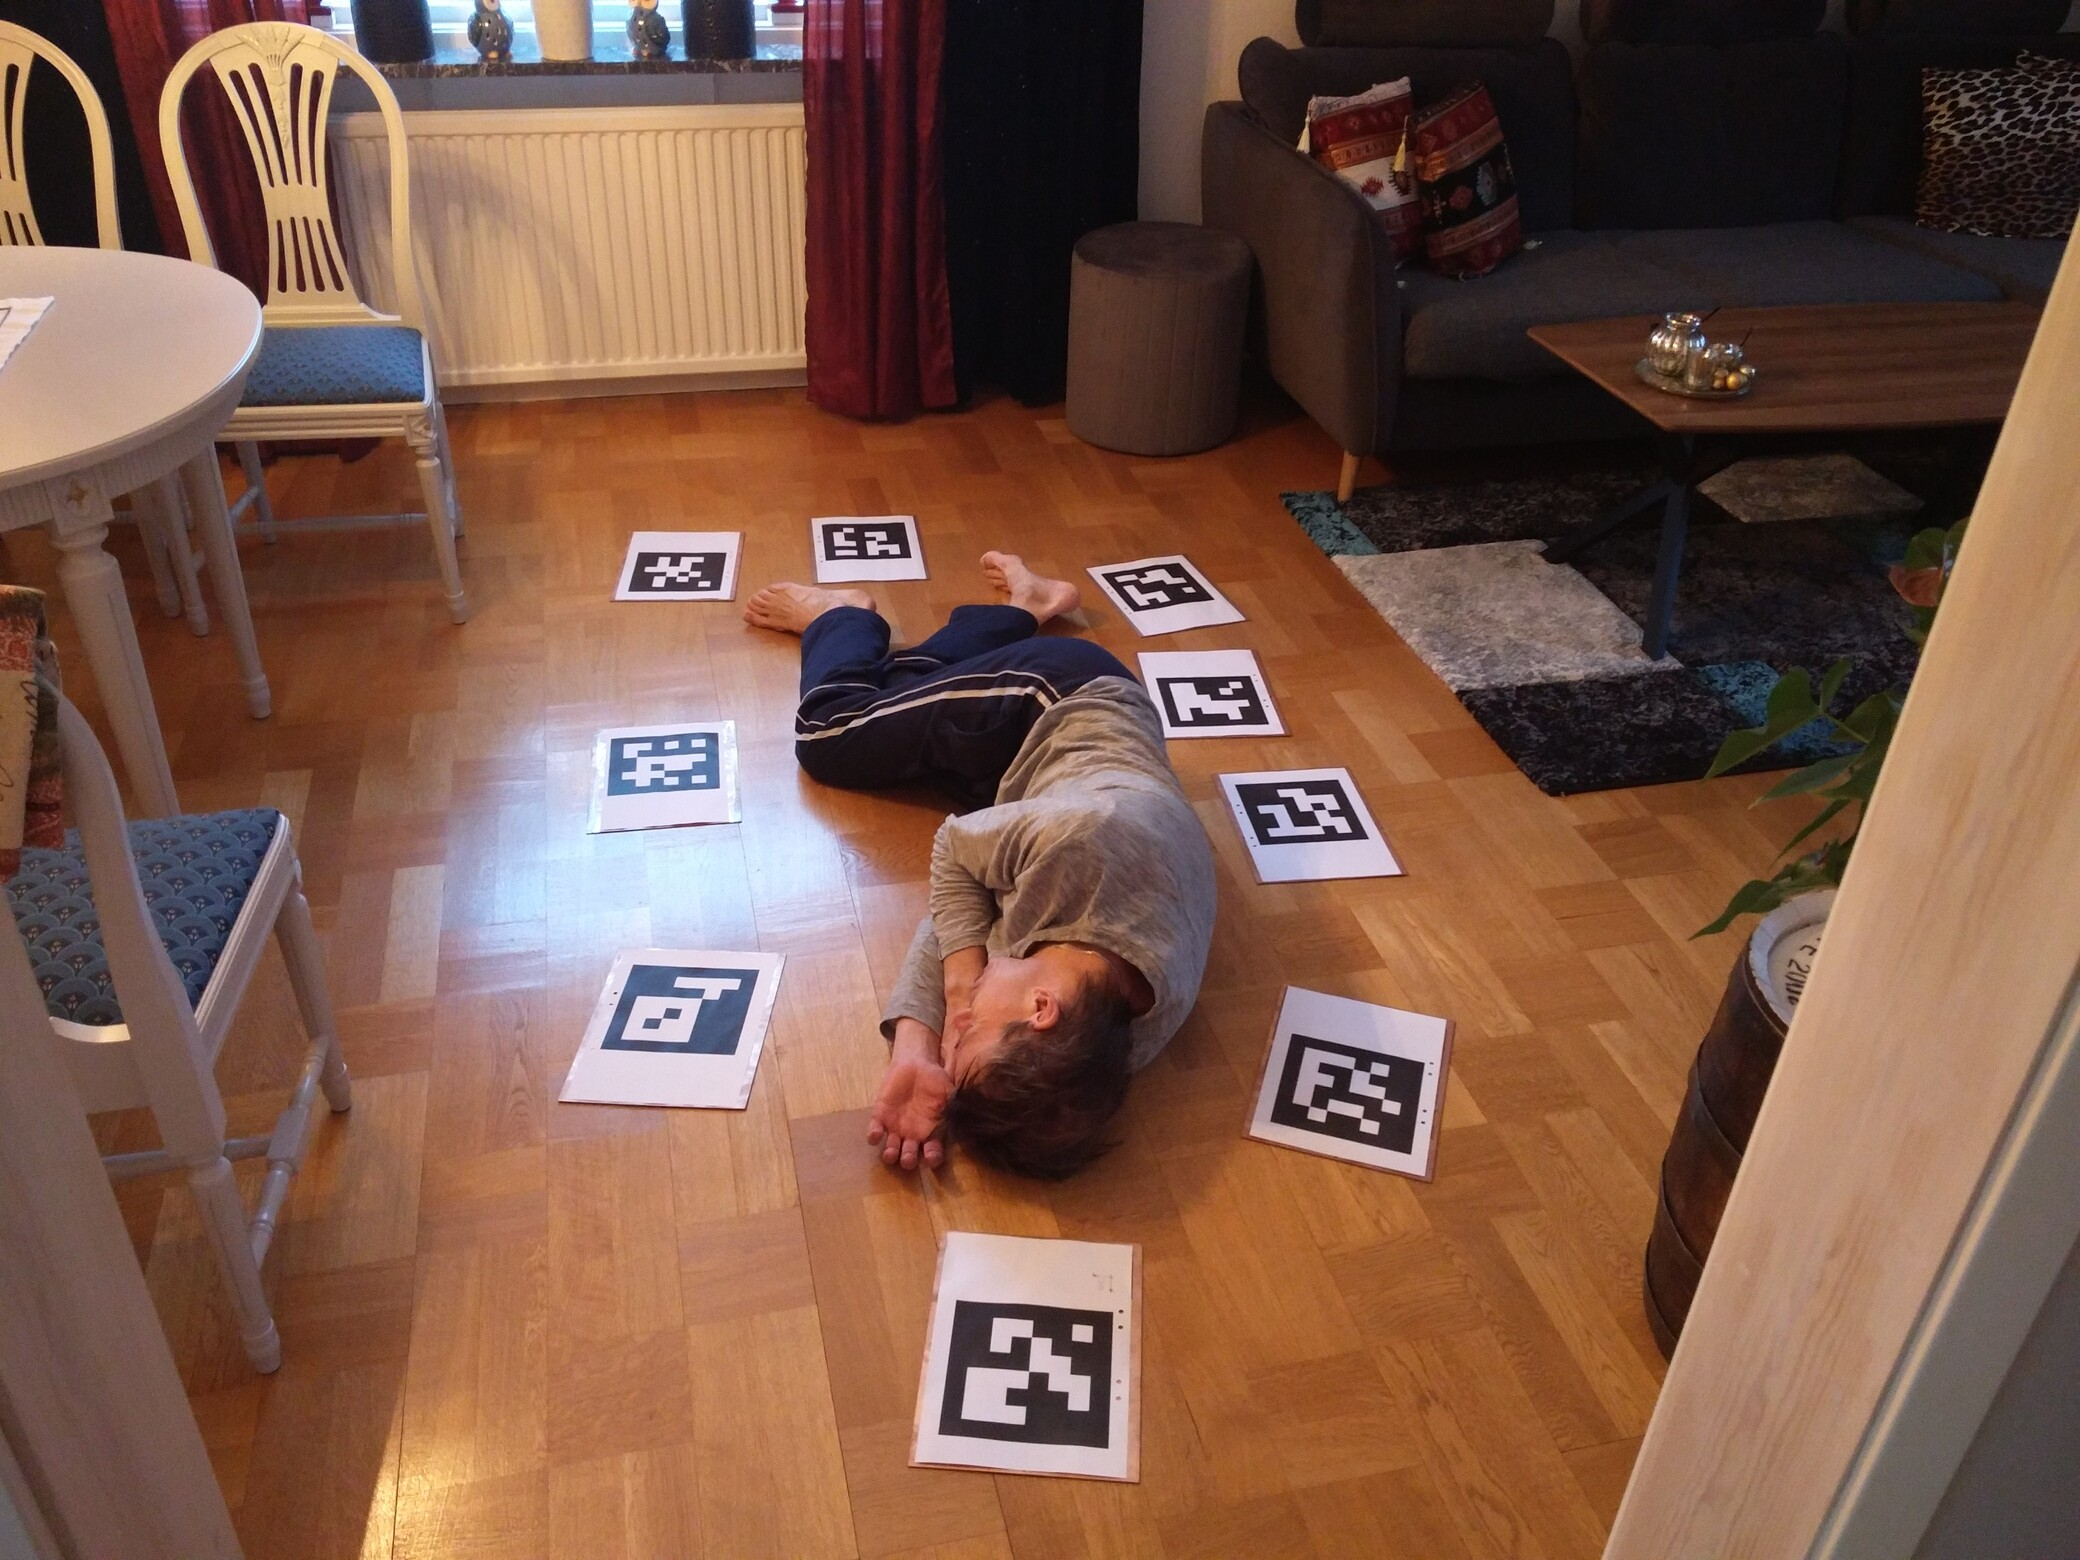
\includegraphics[width=\textwidth]{images/datasets/P2/images/093311.jpg}
        \caption*{North}
    \end{minipage}
    \begin{minipage}[t]{0.2\textwidth}
        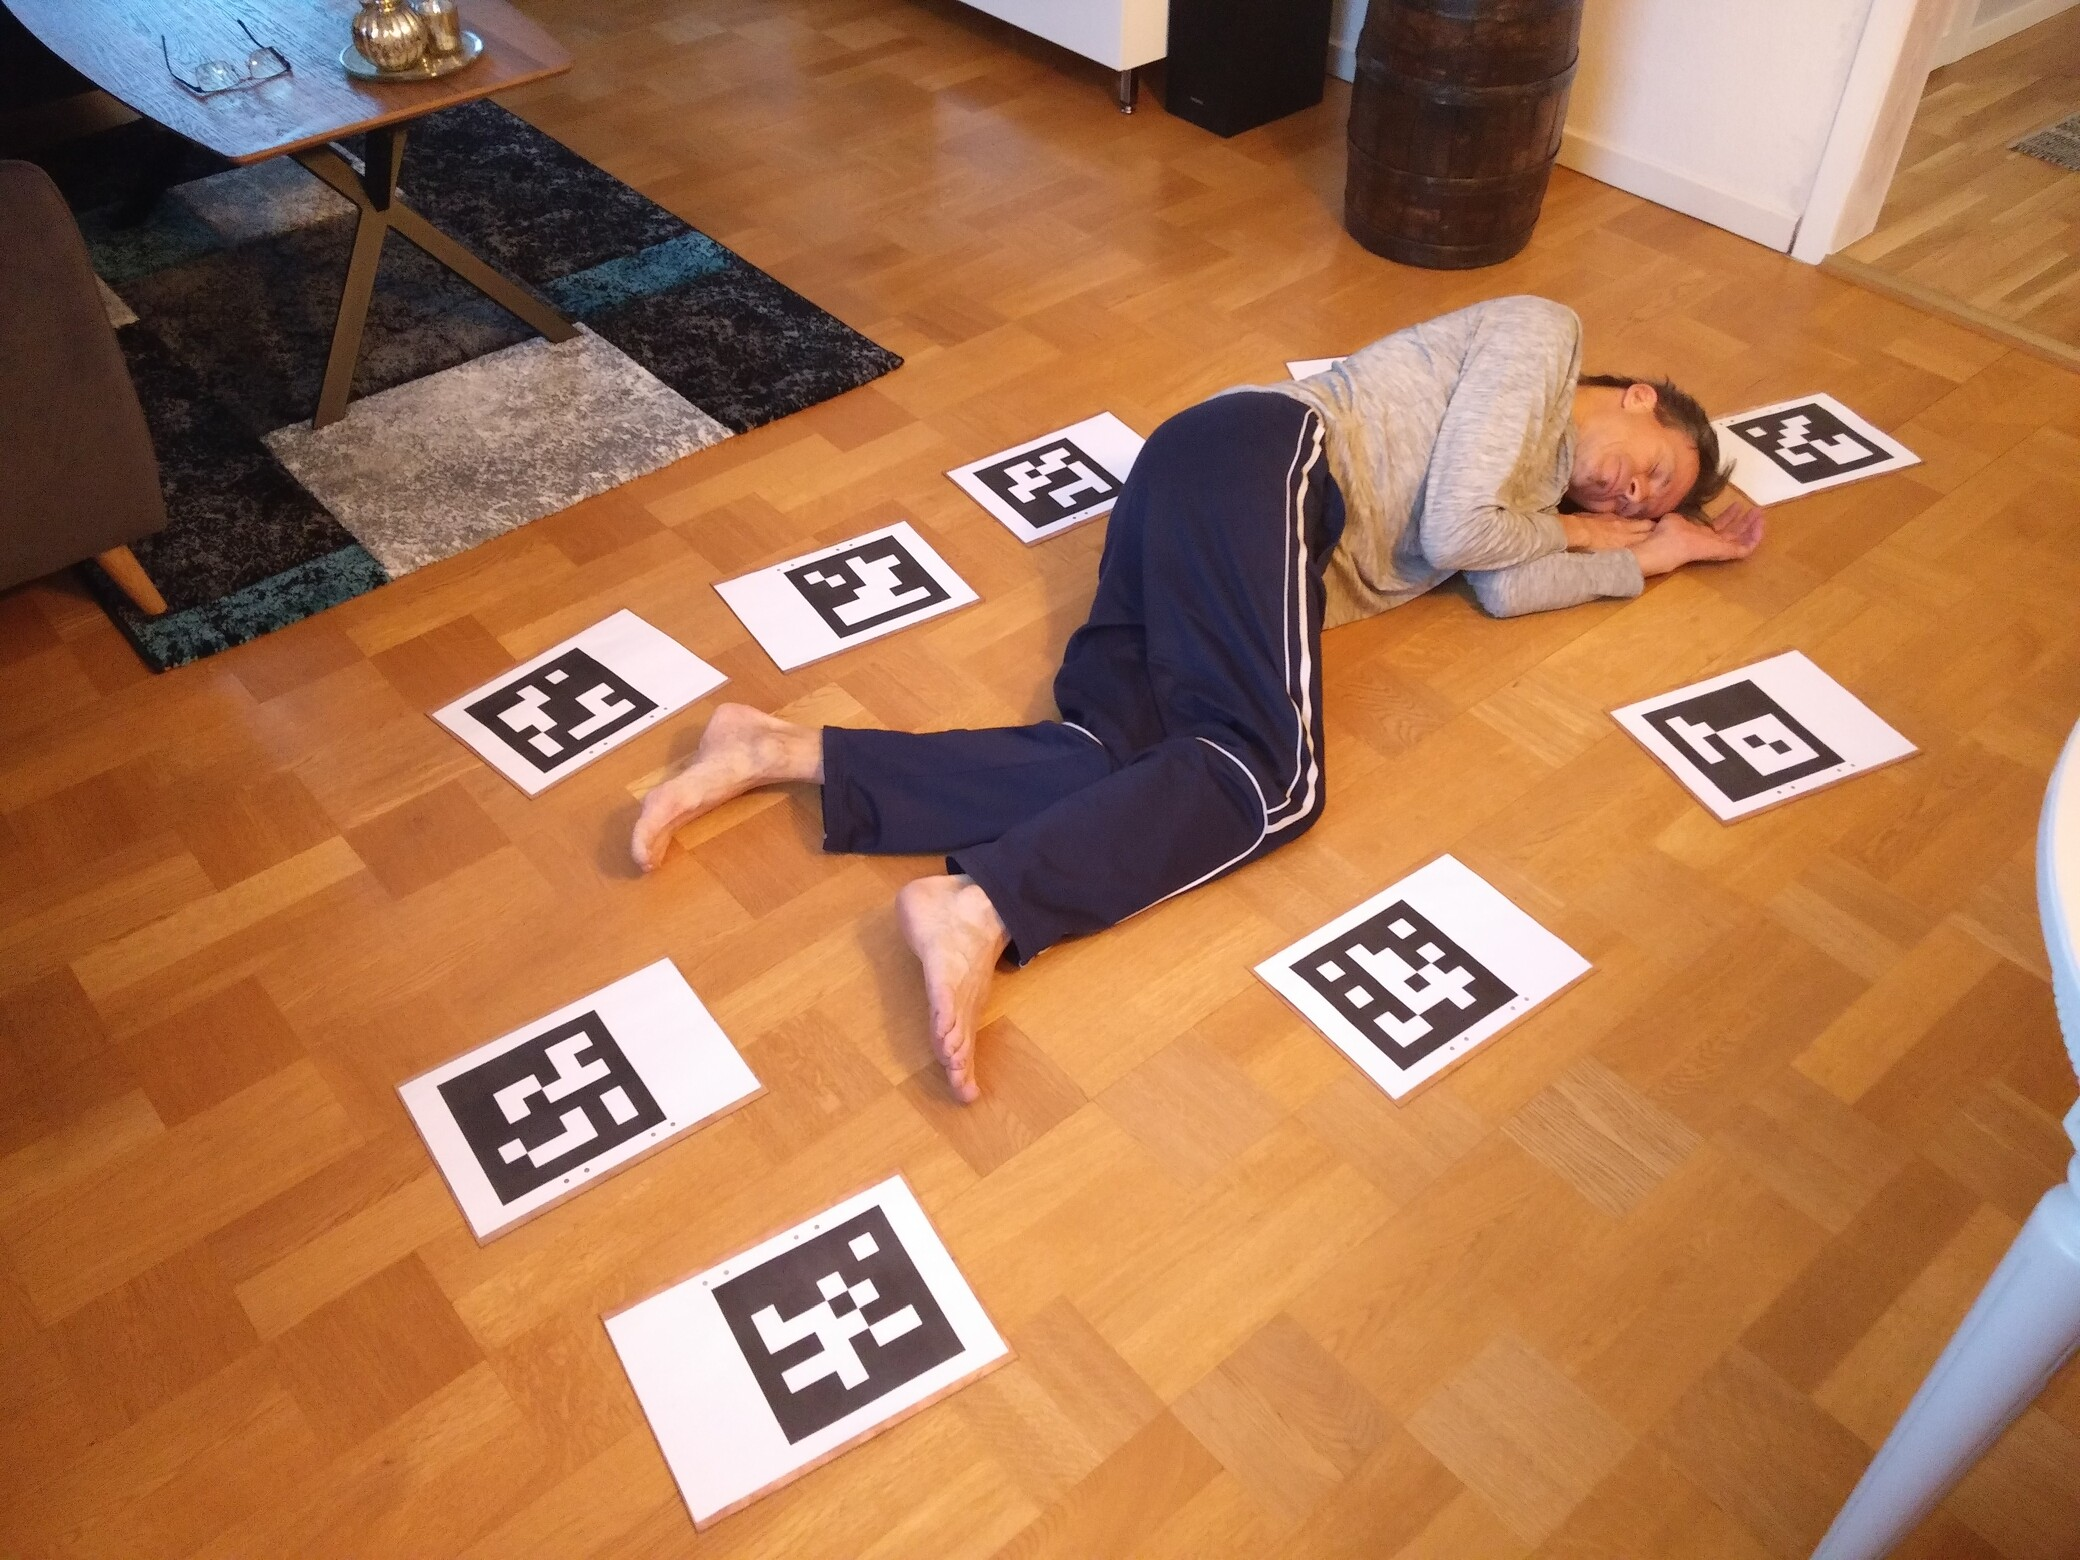
\includegraphics[width=\textwidth]{images/datasets/P2/images/093409.jpg}
        \caption*{East}
        % \includegraphics[width=\textwidth]{pic1}
    \end{minipage}
    \begin{minipage}[t]{0.2\textwidth}
        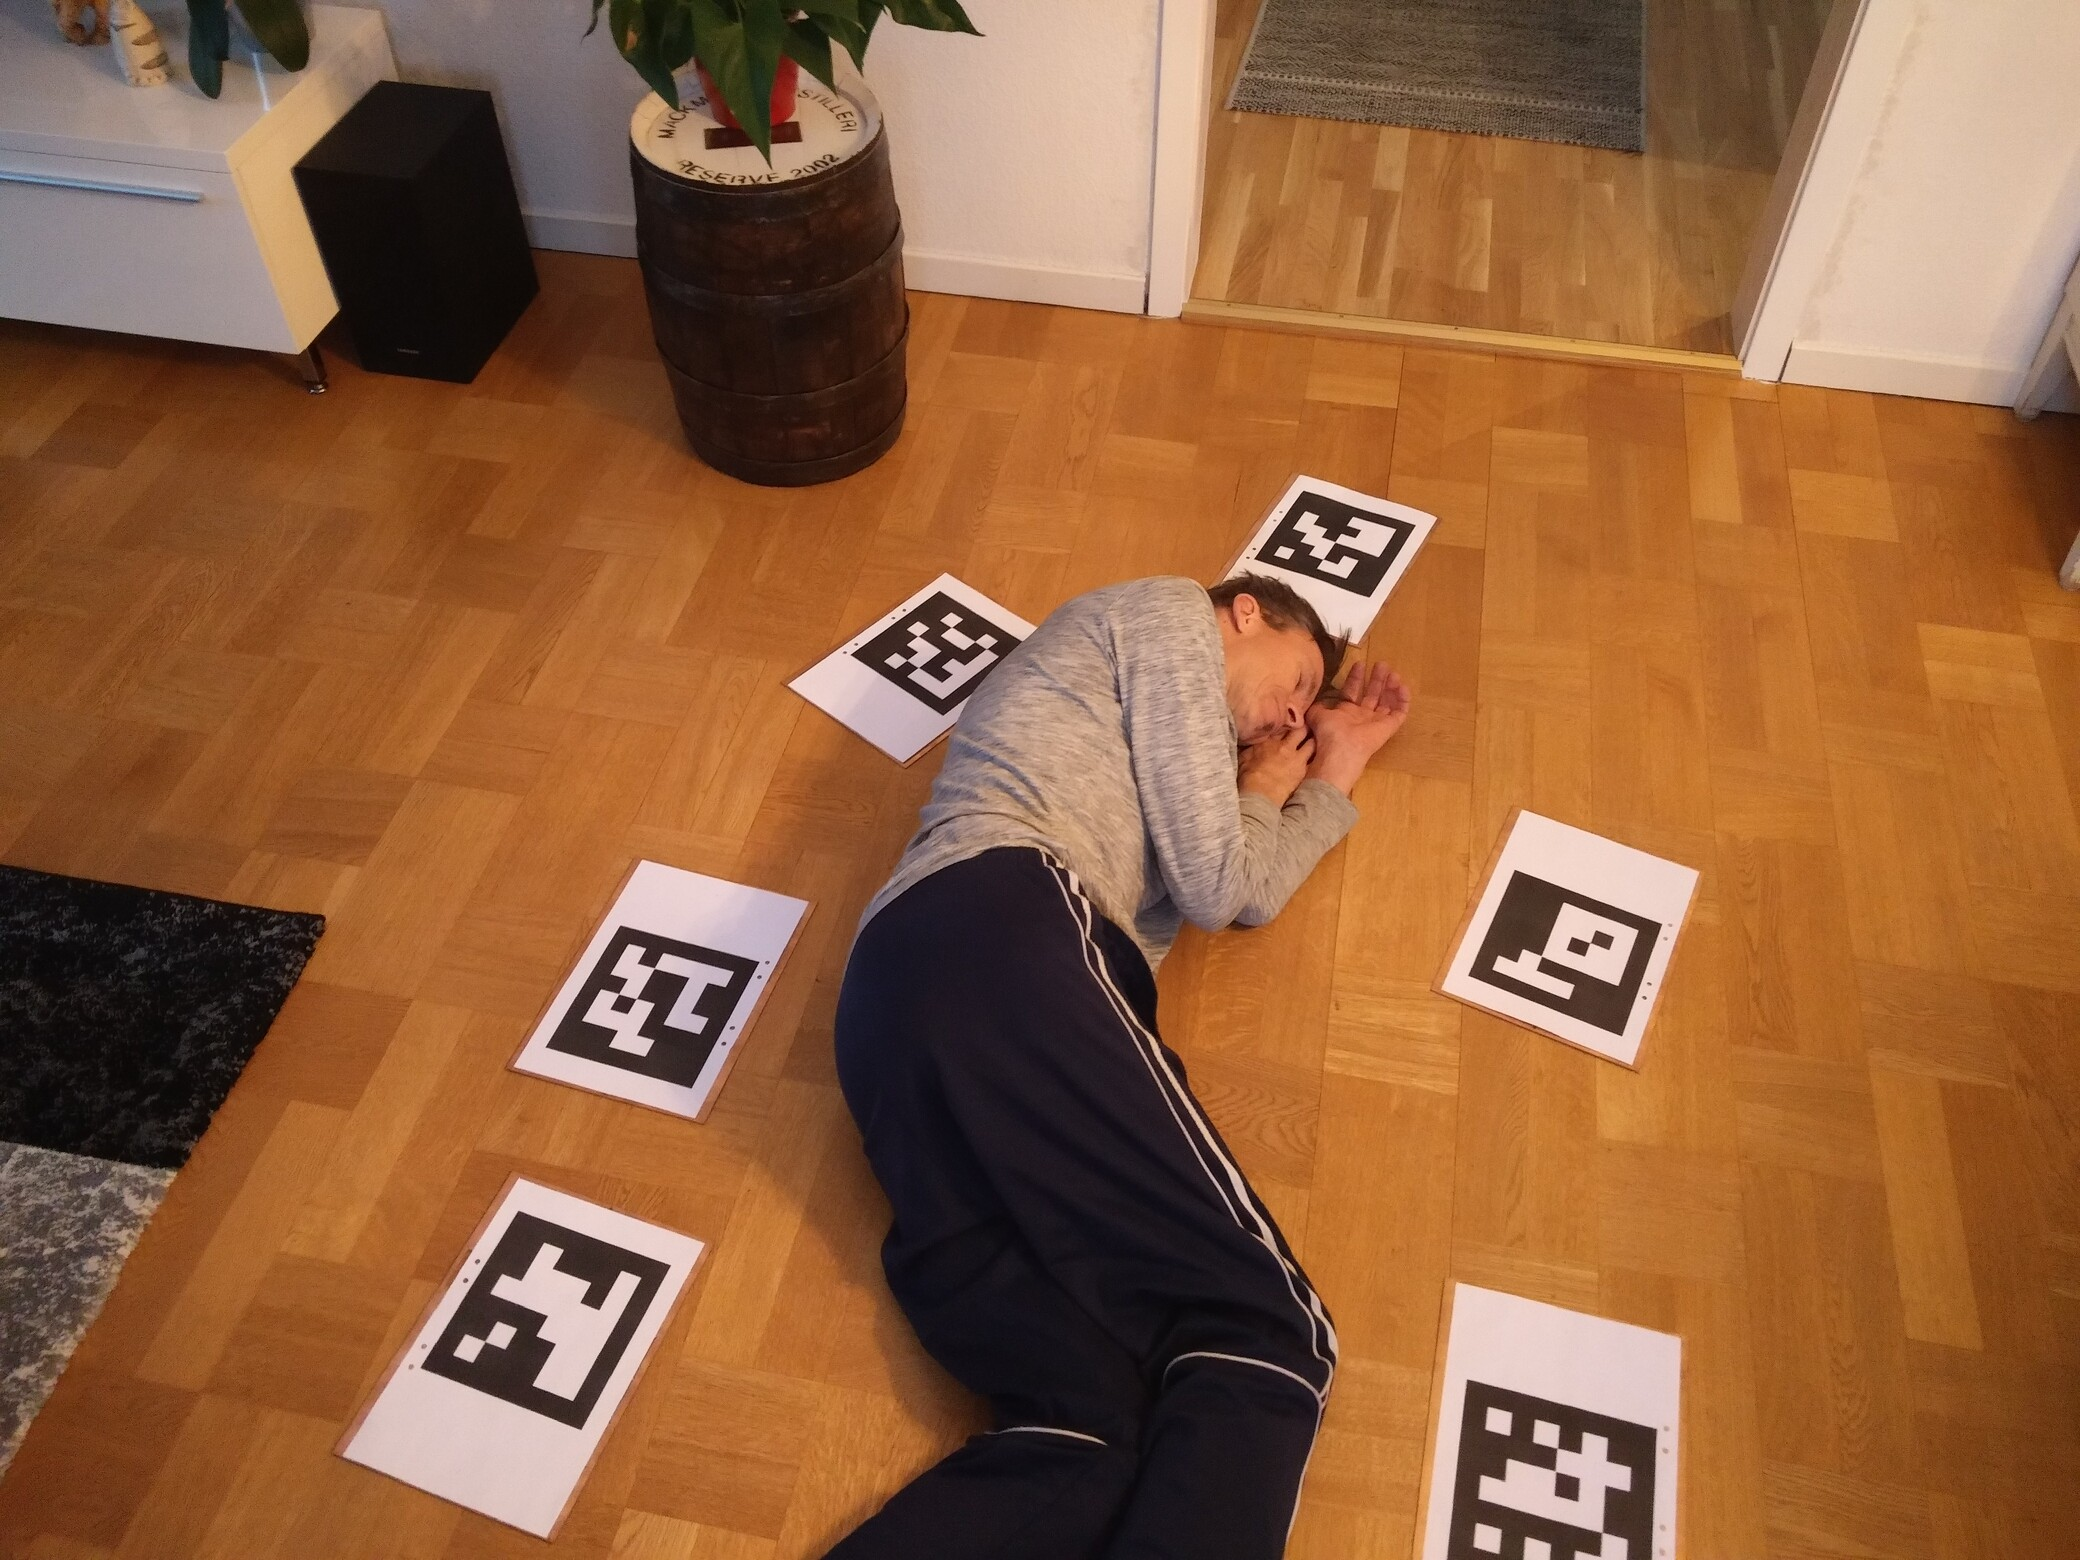
\includegraphics[width=\textwidth]{images/datasets/P2/images/093551.jpg}
        \caption*{South}
        % \includegraphics[width=\textwidth]{pic1}
    \end{minipage}
    \begin{minipage}[t]{0.2\textwidth}
        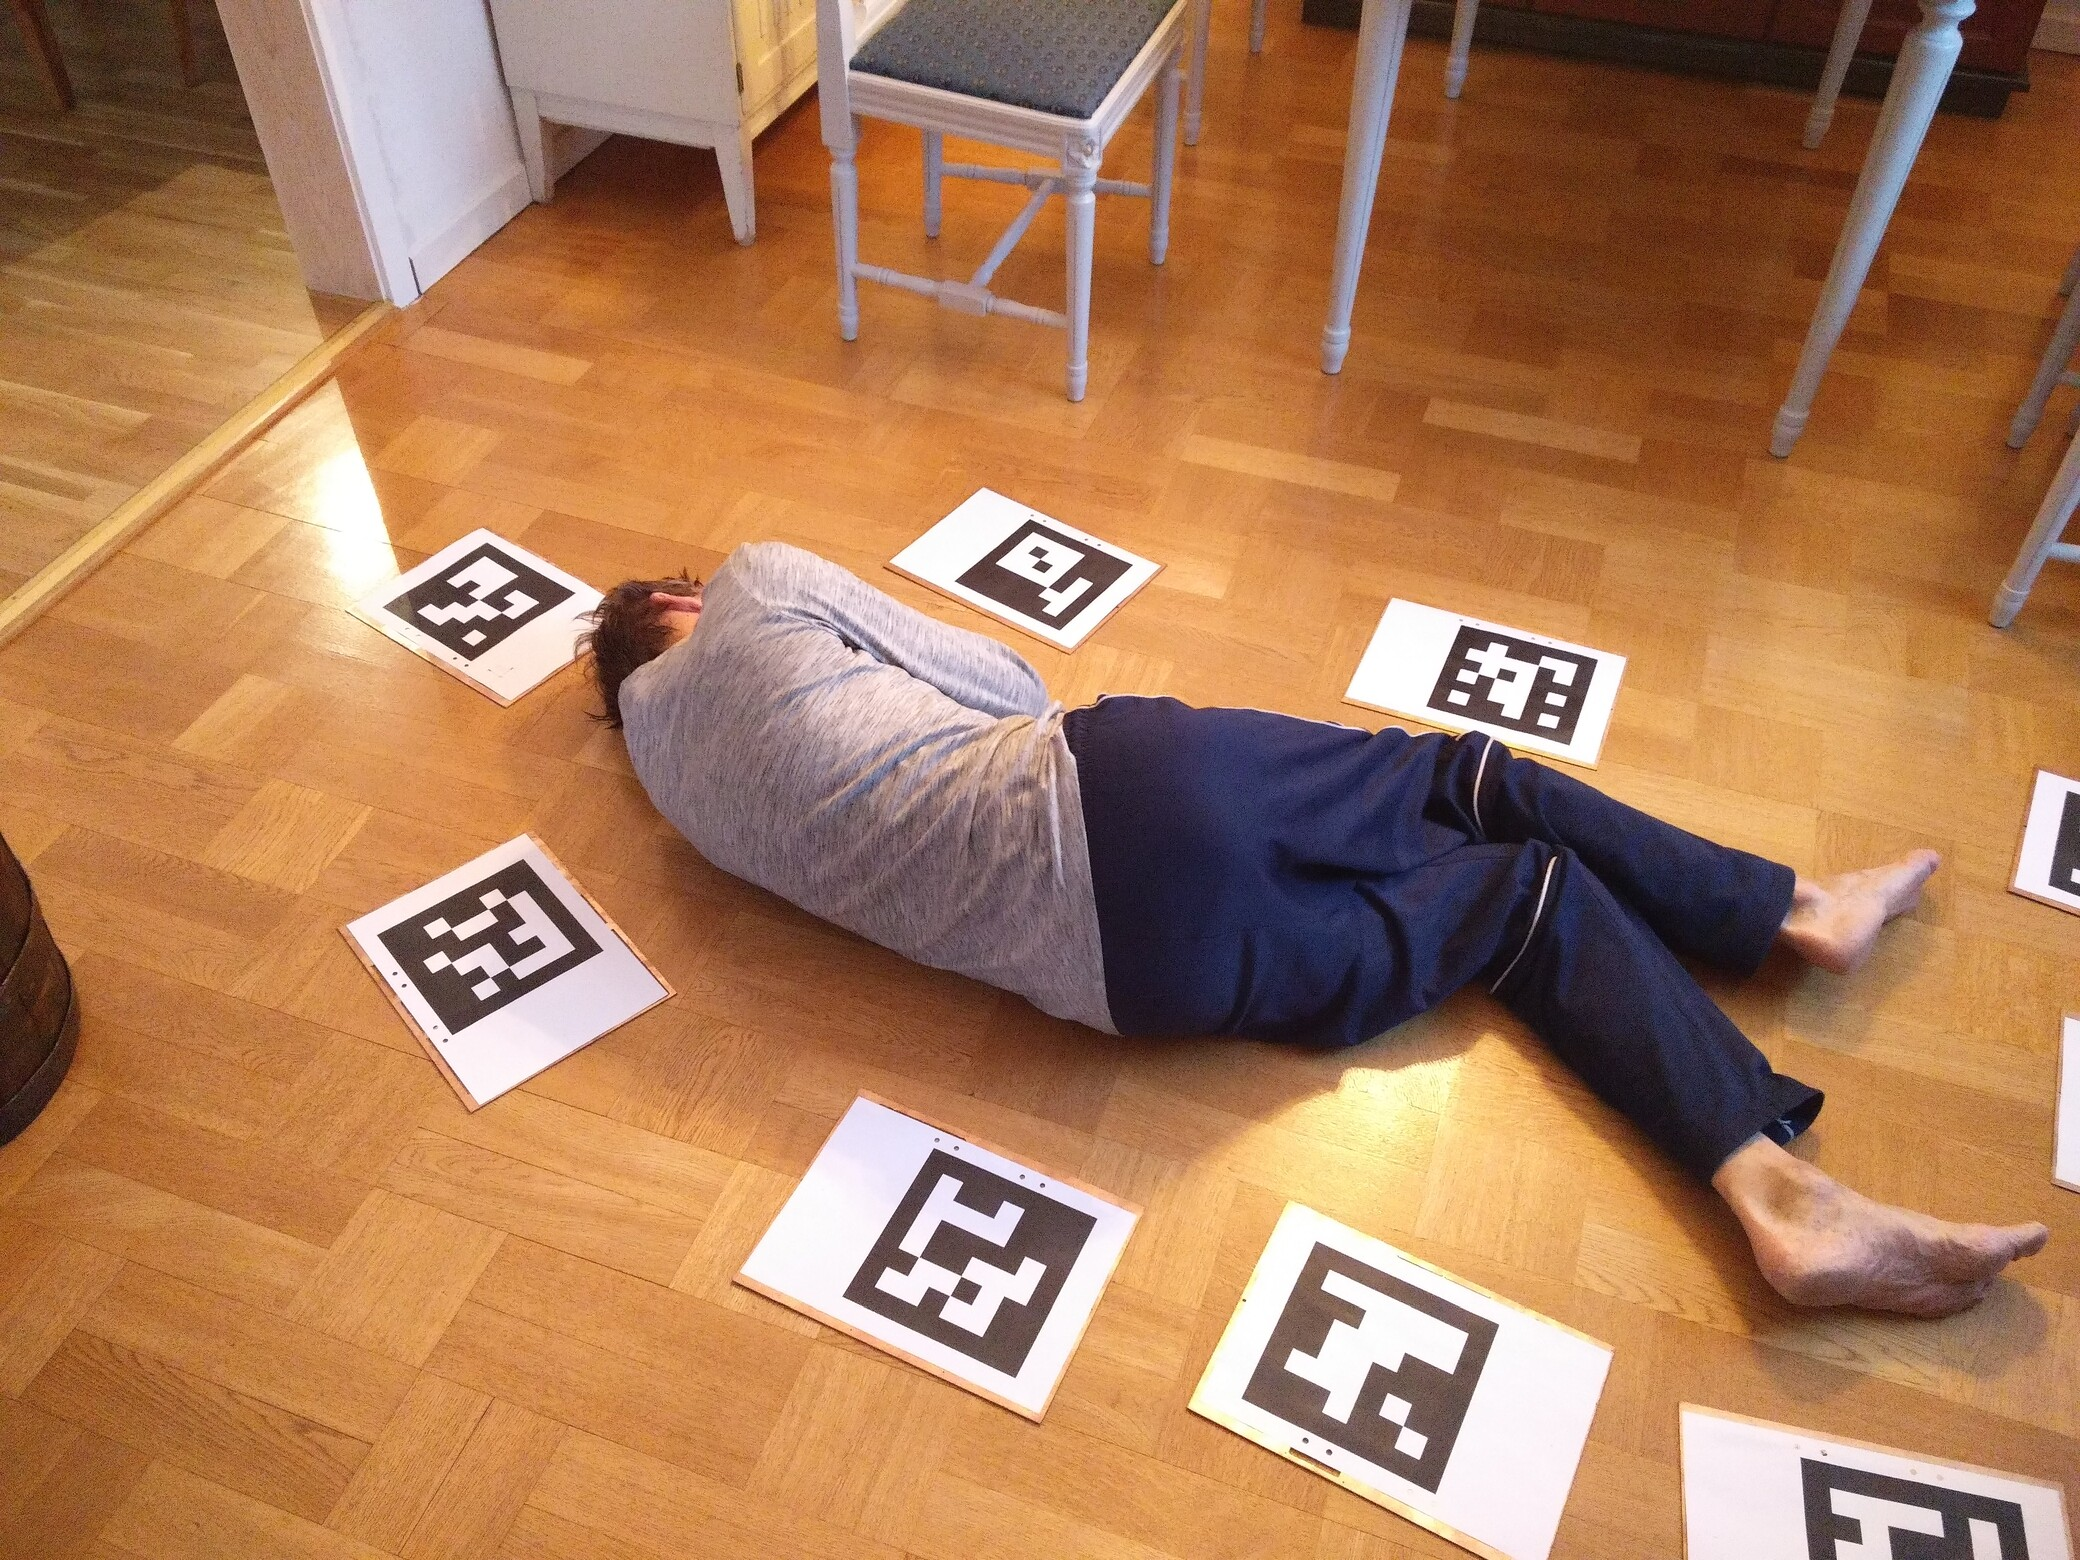
\includegraphics[width=\textwidth]{images/datasets/P2/images/093335.jpg}
        % \includegraphics[width=\textwidth]{pic1}
        \caption*{West}
    \end{minipage}
\end{center}
\caption[Camera quadrant position]{The camera quadrant position in the input set is labeled as follow.}
\label{fig:camera_pos_lables}
\end{figure}

\par

To calculate the total error for all features in every image, first use a subset to calculate the median \(\mu_{u,v}\) for each image and each feature.
Then use that to calculate the total error by taking the Cartesian distance between \(t_{u,v}\) and \(\mu_{u,v}\), who is a feature in a picture with the same label as the selected t variable.
This could be described as the Error equation
% \ref{eq:impl:muerror}.
% \label{eq:impl:muerror}

% \begin{equation} %
% \label{eq:impl:muerror}
% \mu_{error}=\frac{1}{N\cdotm}\sum_{i,j}\Bigg(\sum_{n,m}\bigg(\sqrt{(\mu_i-t_i)_x^2+(\mu_i-t_i)^2}\bigg)\Bigg)
% \end{equation}
\begin{equation} %
\label{eq:impl:muerror}
\mu_{error}=\frac{1}{M\cdotm}\sum_{i}^M\big(|\mu_i - t_1|)\big)
\end{equation}

\begin{align*}
    \text{where:}\\
    % n &= \text{ label } 1\dots N\\
    % N &= \text{ is how many labels there are in the system}\\
    % m &= \text{ image } 1\dots M\\
    M &= \text{ is how many pictures there are in the system}\\
    \mu_{i} &= \parbox[t]{7cm}{\RaggedRight is the median for a particular image,label and coordinate in the system}\\
    t_{i} &= \text{ is one feature to be tested}
\end{align*}
\par
Then the total error from OpenPose to a subset of the human set can be compared with the total error from the human set to its subset using a t-square test.
This error equation is derived from that a regular median for a one-dimensional input is
\[
\mu = \frac{1}{n}\sum_{i=1}^n (x_i)
\]
However, for a matrix, this becomes:
\[
\mu = \frac{1}{n\cdot m} \sum_{i=1,j=1}^{i=n,j=m}(x_{i,j})
\]
Then the internal \(\sum\) is just for building the matrix such that the matrix has \(n\times m\) matrix with the length from the feature to the median.





% \subsection{F-test}\label{sub:implemnt:ftest}
% Before any test can be done the variability of the selected method to test needs to be checked.
% This is done with a F-test and usually a table.
% The first part is using coagulating the ${F}_\text{calc}$
% value that is a score using the standard deviation \sigma of both samples.
% The value must be larger then 1 thus the equation becomes:

% \begin{align*}
% F_{\text{calc}} &= \frac{\sigma^2_1}{\sigma^2_2}\quad\text{if}\, \sigma^2_1 > \sigma^2_2\\
% F_{\text{calc}} &= \frac{\sigma^2_2}{\sigma^2_1}\quad\text{if}\, \sigma^2_1 =< \sigma^2_2\\
% \end{align*}

% Then after $F_\text{calc}$ is found, it needs to be compared with a value
% $F_\text{tab}$ that is usually found in a table if the calculation is done by hand, but in the case of computers, this is derived from libraries, but in this paper, it is still called $F_\text{tab}$ for simplicity.
% \par
% The value for $F_{\text{tab}}$ is derived from the dimension's of the data or how many rows there is in the table for each data set.
% So assume that there is, for example, two sets with the first set have nine rows, and the other set is seven rows. Then the dimension for the F test is $D = (9-1, 7-1)= (8,6)$.
% Using $(8,6)$ in the table \cite[p.~488]{alm2008stokastik} it can be seen that for dimension $(8,6)$ the value is $4,147$
% That means that if our $F_{\text{calc}}$ is lower then
% $F_{\text{tab}}$ then the results are statistically similar to each other.
% That result can then be used to determine if the variance $\sigma$  is equal in both sets, which then determines the t-test category.

% \subsection{T-test}\label{sub:implement:ttest}
% The t-test is a set of tests that will differ based on what data represents.
%\begin{figure}
%    \centering
%    \scalebox{.4}{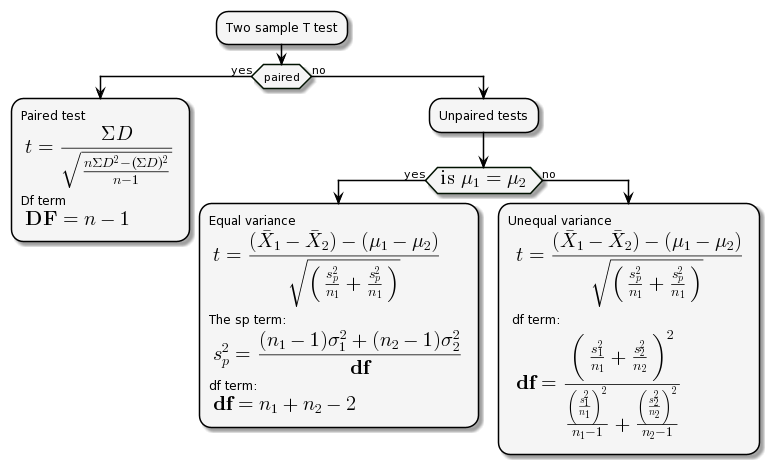
\includegraphics{images/selecting_t_test.png}}
%    \caption{Selecting t test}
%    \label{fig:impl:select_t_test}
%\end{figure}

% \subsection{Verifying the algorithm}%
% \label{sub:Verifying_the_alorithm}
% To verify that the algorithm works as intended, a smaller set of images containing measurable features.
% In this set, it proposed to include a large checkerboard and a few spheres of bright colours to be used as features, and the camera can be mounted to a bracket to be able to intensify the exact location.
% In figure~\ref{fig:validations} a short overview of the system is shown.



% % \def\svgwidth{\columnwidth}
% \begin{figure}[ht]
%     \centering
%         \input{images/validation.pdf_tex}
%         % \input{Figures/validation.pdf_tex}
%       \caption{
%           to be directed in different directions.
%           Future more the tree \aruco corners in the image, scatted on the floor.
%           Also, observe that the \aruco corner $A_0$ can not be followed by camera $C_2$; thus, the camera's position can not be derived directly from $A_0$.
%           However, the position of $C_2$ can be derived by using transfer matrices from the other cameras.
%           In this image, two features marked as $F_g$ and $F_r$ are also present and will be used to validate the system by using the marked checkerboard floor to indicate where the features are in the real world.
%           If the system generates the same features concerning $A_0$ with some scaling factor $\alpha$, the system is valid.
%       }
%     \label{fig:validations}
% \end{figure}


% \begin{figure}
% \begin{center}
%     \includegraphics[width=10cm]{images/uml_outline.pdf}
% \end{center}
% \caption{This figure describes the outline of the project using UML as output layer. At the top the camera with its matrix is shown while the map in the in the bottom is the relation between \aruco corners and camera pose}
% \label{fig:UML_outline}
% \end{figure}



